%% Carl Lindquist
% * <clindqui@ucsc.edu> 2017-03-19T00:28:04.697Z:


\documentclass[]{article}


%----- Packages ----------------------------------------------------------------

\usepackage{graphicx}
\usepackage{mathtools}
\usepackage{amsfonts}
\usepackage[bottom]{footmisc} %push footnotes to bottom of page
\usepackage{float}
\usepackage{xspace}
\usepackage{ragged2e}
\usepackage[letterpaper, portrait, margin=1in]{geometry}
\usepackage[]{hyperref}
\usepackage{color}
\usepackage{listings}


%----- Preamble ----------------------------------------------------------------

\setlength{\RaggedRightParindent}{\parindent}
\def\arraystretch{1.5} % make tables less vertically crammed
\hypersetup{
    pdftitle={CE118 Final Report},
    pdfauthor={Cain Martinez, Babak Khorsand, and Carl Lindquist},
    pdfsubject={Mechatronics Robot},
    bookmarksnumbered=true,     
    bookmarksopen=true,         
    bookmarksopenlevel=1,  
    allcolors=black,
    colorlinks=true,            
    pdfstartview=Fit,           
    pdfpagemode=UseOutlines,    % these are the options you're looking for
    pdfpagelayout=TwoPageRight
}

\lstset{
  frame=single,
  language=C,
  aboveskip=3mm,
  belowskip=1mm,
  showstringspaces=false,
  columns=flexible,
  basicstyle={\small\ttfamily},
  numbers=none,
  numberstyle=\tiny\color{gray},
  commentstyle=\color{gray},
  keywordstyle=\color{blue},
  stringstyle=\color{orange},
  breaklines=true,
  breakatwhitespace=true,
  tabsize=3
}

 
%----- Custom Functions --------------------------------------------------------

\newcommand{\E}[1]{E$\{#1\}$\xspace}
\newcommand{\EM}[1]{\text{E}\{#1\}\xspace}
\newcommand{\ul}[1]{\underline{#1}}
\newcommand{\ol}[1]{\overline{#1}}
\newcommand{\del}{\partial{}\xspace}


%----- The Document ------------------------------------------------------------

\begin{document}
%\RaggedRight % This line stops hyphenation when word wrapping

\title{%
	CE 118 Final Report \\ 
    \large \vspace{3mm} Luke SkyScraper: The Last SlugI}
\author{Babak Khorsand, Cain Martinez, Carl Lindquist}
\date{\today}		% leaving the brackets empty omits the date
\maketitle
\(\)


%===============================================================================
%===== The Sections ============================================================
%===============================================================================
\section*{Introduction}
The motivation for this project was to showcase all that we have learned while taking CMPE 118 and applying ourselves to solving an open ended problem. 

Our team was tasked to build an autonomous robot that could navigate a standardized game field. The robot had eliminate three randomly placed AT-M6 targets using its ping pong ball ammo. Once all three targets were down, an IR beacon illuminated, indicating the location of Kylo Ren's ship. The robot then had to shoot down Kylo Ren's ship with a precise shot.

We had 31 days to complete the task.

\section*{Rules and Regulations}
The game field is a 4'x8' in white surface with 2" tape marking the boundaries. The three randomly placed AT-M6's are 8" wide and 12" tall. The hole is 4" in diameter. They are marked with a track wire which runs vertically down the surface at 25kHz. Targets are destroyed by putting a ping pong ball through the hole in the target. There are no restrictions on the method of delivery.

Once all AT-M6's are eliminated, Ren's IR beacon illuminates with a frequency of 2kHz. Rens ship is at the end of the game field with a black tape "T" marking its location. Ren's Ship stands at 16" tall and 12" wide with a set of fiducial alignment holes on its surface. The target hole is centered at 14" and is 2" in diameter.

At the beginning of the game, the beacon will be on for 15 seconds, and then will turn off for the remainder of the match until all three AT-M6's have been eliminated. There will be a randomly placed obstacle (which could be up to 11"x11"x11") and collisions with the obstacle have to be resolved within 5 seconds or face disqualification. The robot has to eliminate all AT-M6 targets and the Ren ship within 2 minutes.

The robot must fit in an 11"x11"x11" box at the beginning of the round and must contain all possible ammo at the start of the round. No reloading is allowed during the round. It can only draw power from batteries and must be able to detect bumps with an obstacle at 3.5" above the ground and resolve crossing obstacle tape in the middle of the field. The robot has to be equipped with a remote power switch and has to be programmed in C. 
There is a budget for the project, which should not exceed 150 dollars. all work has to be done by the team and not contracted out. all circuits MUST be soldered on perfboards. This means no breadboards.

\section*{Mechanical:}
\subsection*{\textit{Introduction}}
The mechanical design process is where we came together as a team to brainstorm and prototype the body and delivery mechanisms for our robot using Solidworks. Through the process of incremental design we were able to come up with a model which could complete the task.

\subsection*{\textit{Methods and Materials}}
The Materials used:
\begin{itemize}
    \item \text{24" x 24" x 1/4" MDF boards}
    \item \text{24" x 24" x 1/4" foam-core boards}
    \item \text{clear 1/4" acrylic sheet}
    \item \text{2 rubber wheels} 
    \item \text{8" long, 1/2" diameter steel threaded bolt}
    \item \text{2 Steel washers}
    \item \text{5, 3/4" hexagonal nuts}
    \item \text{1, 10kg-cm torque servo motor}
    \item \text{2 9g servo motors}
    \item \text{3 12V DC brushless motors}
    \item \text{2 metal motor mounts}
    \item \text{screws and nuts}
    \item \text{Glue gun}
    \item \text{heat shrink}
    \item \text{5 Mechanical switches}
\end{itemize}

The mechanical design began with all team members brainstorming about how the robot would move around and how to launch ping pong balls. After some discussion, we settled on the idea of the bot changing height mid-round, to match the target, then simply have the ping pong balls roll in. The balls would be held in a hopper that would be resting at an angle so the balls are tilted down. The majority of the bot was made using medium density fiber board (MDF), with small amounts of acrylic and foam-core. 

The next part consisted of discussing how the height of the bot would actually change, as well as where the IR tape sensors would be placed. We eventually settled on changing height by using a DC motor to spin a captive nut, moving a bolt vertically; the bolt would hold the top platform in place using washers and two more hexagonal nuts on both sides(top and bottom). Eventually this evolved further into a gear drive with no belt, where a large driver gear spun a smaller driven gear which in turn had the hexagonal nut cut in, and the bolt was moved up and down in the same fashion. To prevent the bolt from spinning, two hex nuts were locked together and aligned, and a triangular sleeve was cut to house the bolt. The sleeve prevents the nuts and the bolt from spinning.

\begin{figure}[H]
    \centering
    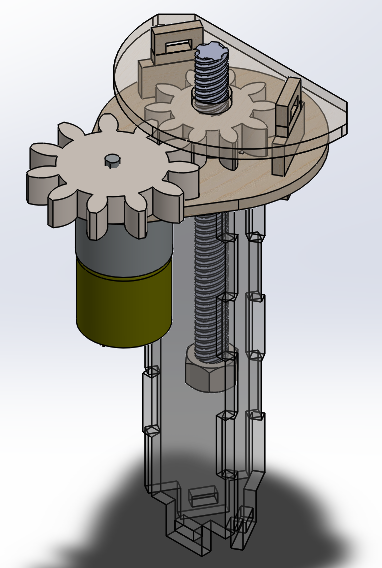
\includegraphics[scale=0.50]{lift-CAD.PNG}
    \caption{The sleeve and the top plate have been made transparent to see the bolt and gears.}
    \label{lift cad}
\end{figure}


We then moved onto discussing the tape-following algorithm, this allowed us to plan the tape sensor locations. The sensors used were the Vishay TCRT5000 IR sensors, and were originally placed in a triangular arrangement centered about the middle of the bottom plate. The front sensor alone would follow the inside edge of the tape, while the other two were for detecting corners. Eventually we decided to move the front most sensor closer to the front of the bot, which gave use much greater tape-following accuracy. The new arrangement had each sensor at the vertex of an isosceles triangle and are shown in the figure below.


\begin{figure}[H]
    \centering
    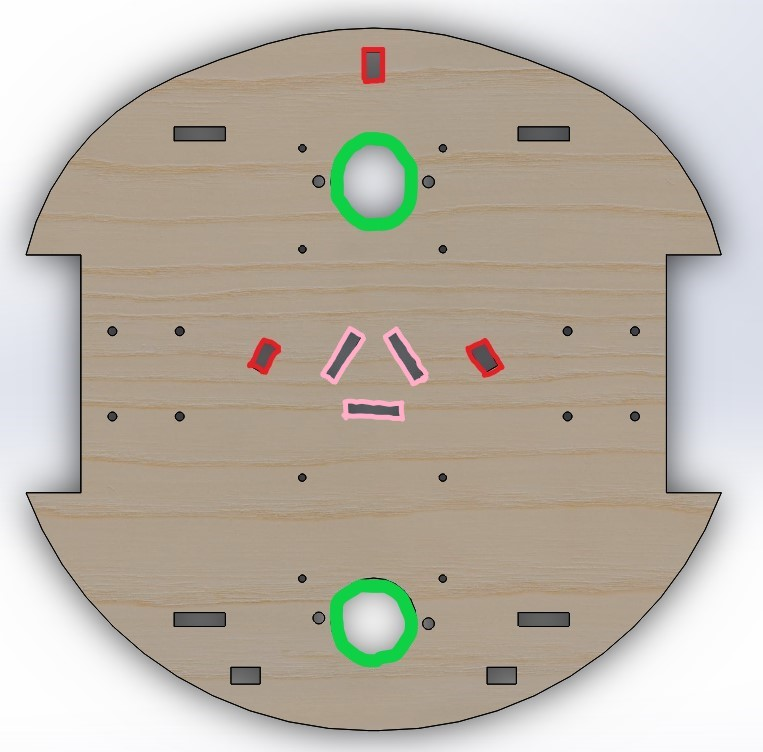
\includegraphics[scale=0.45]{bottom-plate-highlight-CAD.jpg}
    \caption{Note the tape sensor locations highlighted in red, ball caster locations in green, and bolt sleeve tab slots in pink.}
    \label{bottom plate highlight}
\end{figure}


The next steps were to discuss balancing the robot, the bumper plates, aligning the top platform, and what type of motors to use. The bottom plate of the robot first began as a pentagonal shape. Then the side cuts were included to bring in the wheels, various screw holes were added, and the overall shape started to become much more rounded to reduce the possibility of snagging on objects.

Shown in Figure \ref{bottom plate highlight} are two circles (highlighted green) for the ball-casters used to balance the robot so that it wouldn't tilt forward or backwards; ball-casters were used instead of skids to reduce friction when moving around. The cut-in squares on the sides of the plate are where the rubber roller-skate wheels were placed. We connected the wheels to the DC motors with acrylic plugs cut to fit tight with the motor shaft. The DC motors themselves were screwed into metal mounts, which were then screwed in the set of four 1/10" screw holes near the sides of the plate. With both the wheels and ball-casters in place the height difference between the bottom of the casters and bottom of the wheels was less than 1/10" so the robot was well balanced with a small tilt. Around the top and bottom ball-caster cut outs were sets of four 1/10" screw holes which were used to hold the two H-bridges in place. The first prototype of the bottom plate was simply a foam-core cutout with the tape sensor positions. This allowed rapid changes to the layout, and for us to easily move it around the field. 

Centered at the middle of the plate, are another set of three cutouts forming a triangle, these cutouts are highlighted in pink. Looking back at Figure \ref{lift cad}, there are tabs sticking out the bottom of the sleeve, which fit into the cutouts previously mentioned, and keep the sleeve in place. The tabs also have smaller MDF thick cuts that are for pins which help keep the sleeve in place. 
When first considering the bumper plates, a small platform was planned sticking out of the front of the bottom plate; this small protruding platform had both the collision and the fiducial bumpers resting on it. However, as the design progressed and the group began considering the placement of all the components. This small platform was extended and became an entire second level plate which had space for the UNO stack, bumpers, switches, and some circuitry. The circuitry placed on the second level included the track-wire sensor circuit as well as the switch distribution board. 

Collisions with the robot were detected using switches placed behind bumpers, when hit the switch would go high and there would be a voltage high reading at the appropriate UNO pin. Switches were also used to correctly line up with the final target, as there were fiducial holes at certain heights, these bumpers were placed at an appropriate height and position such that when aligned, both of their switches and the collision bumper switches would be pressed. These bumper plates ended up sitting 3.5" off the floor to the bottom of the plate for the collision bumpers, and approximately 5" off the floor for the fiducial bumpers. Another switch was also used as an indicator to know when the height changing mechanism had reached the lowest point. This was significant because it served as an indicator for the micro-controller about the bots height, using it as a reference on start-up. A back bumper plate was also planned but was never implemented as there was no need to. The bottom plate of the bot also included the battery and the IR sensor distribution board. The final model of the lift mechanism, and the first two levels are shown in Figure \ref{no upper platform cad}. 

As shown in Figure \ref{no upper platform cad} above, the second level was held in place by a pair of arches positioned at the front and rear of the robot. The rectangular piece on the left with the circle cut out near the top was used as the stand for the inductor used in the tank circuit of the track-wire sensor. 

\begin{figure}[H]
    \centering
    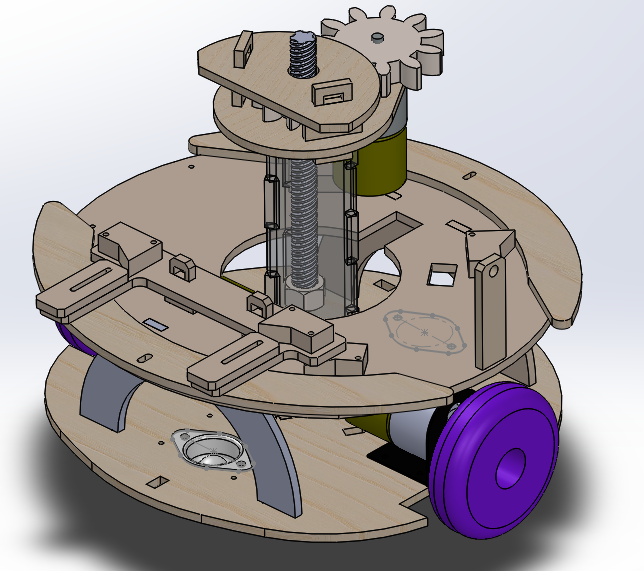
\includegraphics[scale=0.50]{bottom-platform-CAD}
    \caption{The top level shows the T hopper along with the bridge and detent servos}
    \label{no upper platform cad}
\end{figure}

This led us to plan out our top level, which would be our method of delivering ping pong balls to eliminate the targets. We felt that shooting the ping pong balls from a launcher would introduce various forms of error, which culminated in us ruling out an actual launcher for delivery. This led us to a more simplistic approach of simply "handing" the balls over to the target via bridge, which drew and dropped with a servo.

The balls were held in a "T" shaped hopper with separate ends going to separate targets. The "T" had one opening that was facing the left of the robot, which was exclusively for AT-M6's. At the end of the opening there was a servo that drew and dropped the bridge for delivery. At about 2" from the opening, there was a detent servo which was timed just right to only allow one ball to be delivered at a time. There was another opening on the "T" facing the front of the bot.This one, with another detent servo. Upon alignment with the Ren ship, the servo would open and drop both ping pong balls into the target. The four balls would be held in single-file to be delivered to AT-M6's along the longer line, and two balls would be delivered to Ren along the shorter line. The second ball was there to ensure against the ball not having enough momentum to go all the way into the Ren ship.

The bridge was a small piece of MDF that was about the length and width of the servo arm. Attached to it with heat shrink was a skewer about 3 inches in length. We added joints in the skewers using heat shrink tubing. The flexibility of the bridge was an essential part of our delivery method to prevent the bridge from breaking when contact was made with an AT-M6. To get the ball to actually roll off we needed to add another flexible MDF-skewer arm. These had to be held together at ball length with a "V" shaped component we called the "Chevron"

The Chevron was shaped exactly as the name implies. The shape was not for aesthetic purposes. It was intentionally designed in a way where we maintained the MDF-skewers fixed with respect to one another, but also did not impede the ball from rolling down. The Chevron alone was not enough to stabilize the bridge so a straight piece of MDF was glued to the back end of the bridge.

The detent servos required minimal assembly. They consisted of a single popsicle stick which was cut to be about 3" which was heat shrunk onto the servo arms. The shooting mechanism is shown below in Figure \ref{Top level}

\begin{figure}[H]
    \centering
    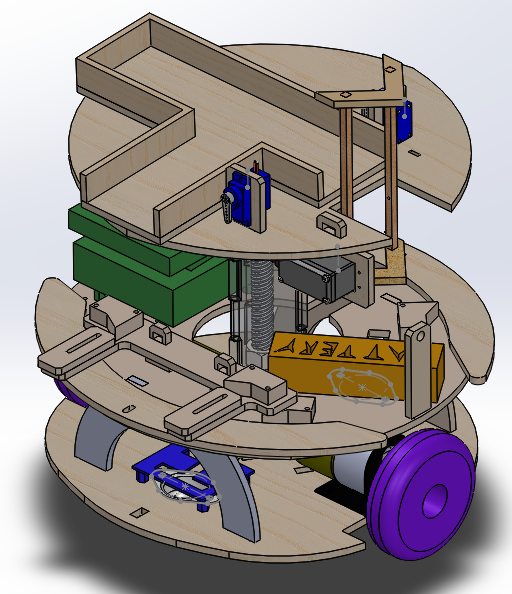
\includegraphics[scale=0.50]{Luke-CAD.PNG}
    \caption{The top level shows the T hopper along with the bridge and detent servos}
    \label{Top level}
\end{figure}


\subsection*{\textit{Setbacks}}
There were various setbacks when prototyping the robot. The major mechanical problems involved the height changing mechanism, and corner cases involving collisions. After going through and testing various forms of driving the bolt up and down, the problem of slipping and stalling persisted, with a belt drive the belt would end up sliding off and the wheels would disconnect, the friction fit could not be done well enough such that it would perform consistently without stalling or slipping. Eventually the team settled on using a gear interface with a driver and driven gear because it had the least chance of the driver and driven components to lose contact.
One of the major setbacks faced involved rare collision cases when the robot collided with the obstacle at a particular angle. At this angle it doesn't hit the fiducial bumpers, and strikes the collision plate such that the switch isn't pressed. So while the robot is stuck it can't realize it. The first solution was to shave the top right and left of the bottom plate because they were slightly less curved than appropriate in that they stopped the bot before the bumper could fully go in. This solution worked half the time, this is because at other instances the obstancle would get caught on the support plate under the ficudial bumpers, so again parts of the support platform sticking out the front was shaved to curve out the inside to help slide the collision until the bumpers are pressed. 

Another setback regarding the size of the bottom platform appeared during test to align with the final target. The issue was when trying to align with the final target and press fiducial bumpers, the tip of the bottom plate was sticking out too much and one of the bumpers would remain unpressed. To fix this the tip of the bottom plate was rounded out.

The issue that consistently plagued us however was the breaking bridge. Because the bridge servo motor was so powerful, every time the robot was turned on or off if the bridge was stuck or obstructed in any way, it would break. Eventually this led to the multi-joint bridge solution which bent at the joint to prevent the bridge from breaking again.

\subsection*{\textit{Results}}
The end result of the mechanical design is what is illustrated in Figure \ref{Top level}. The bottom of the bot rested 3/5" above the floor, and while not shown in Figure \ref{Top level}, a paper skirt was added to the front and back of the bottom plate to reduce noise for the tape sensors. The robot stood at a little over 10" tall, 9.5" wide, and 9.5" long, and had three levels. The majority of the components rested on the first and second levels, with two boards connected to the underside of the top plate. 

\section*{Electrical:}
\subsection*{\textit{Introduction}}
This section covers the electrical modules that were needed to detect the track wire inside the AT-M6's, a module that detects the IR signal coming from the beacon, and power distribution modules for the tape sensors, as well as bumper and servo power distribution modules.
\subsection*{\textit{Methods and Materials}}
The Materials used:
\begin{itemize}
\item\text{5 x Various Size Perfboards}
    \item\text{5 x Female Molex Connector}
    \item\text{9 x 10nF capacitor}
    \item\text{6 x 0.1uF capacitor}
    \item\text{22nF capacitor}
    \item\text{3.3 nF capacitor}
    \item\text{2 x LM1086 3.3V regulator}
    \item\text{PhototDarlington}
    \item\text{2 x DIP14 Sockets}
    \item\text{2 x MCP6004}
    \item\text{Various resisters}
    \item\text{LED}
    \item\text{1 x 10mH inductor}
    \item\text{3 x KY5033 3.3V regulators}
    \item\text{7 x Diodes}
    \item\text{Female Headers}
    \item\text{Male Headers}
    \item\text{wire}
    \item\text{Solder Iron}
    \item\text{Solder}
    \item\text{Heat shrink}
\end{itemize}
Once we were set on the general structure of the robot we began the process of designing and making the modules that would give it information about its environment. These modules were: The trackwire detector, beacon detector, bump sensors, and tape sensors, along with the power distribution boards, which provided a centralized and convenient place to allocate sensors. The power distribution boards were also key to wire management on the robot. Each distribution board had it's own 3.3V regulator and was powered by the UNO power shield; on the distribution boards there were output pins as well which connected to the UNO I/O shield. This way seemed to provide the cleanest solution to deliver power to the sensors, and provide input to the microcontroller. 

The most complicated parts were the trackwire and the beacon detector. The trackwire detector was designed to pick up the 25kHz signal from AT-M6's when the robot was approximately 6" from the left side of the bot, but the close proximity to the wheel motors added some 30kHz noise. The solution here, was to design and add an active filter to isolate the trackwire signal.

\begin{figure}[H]
    \centering
    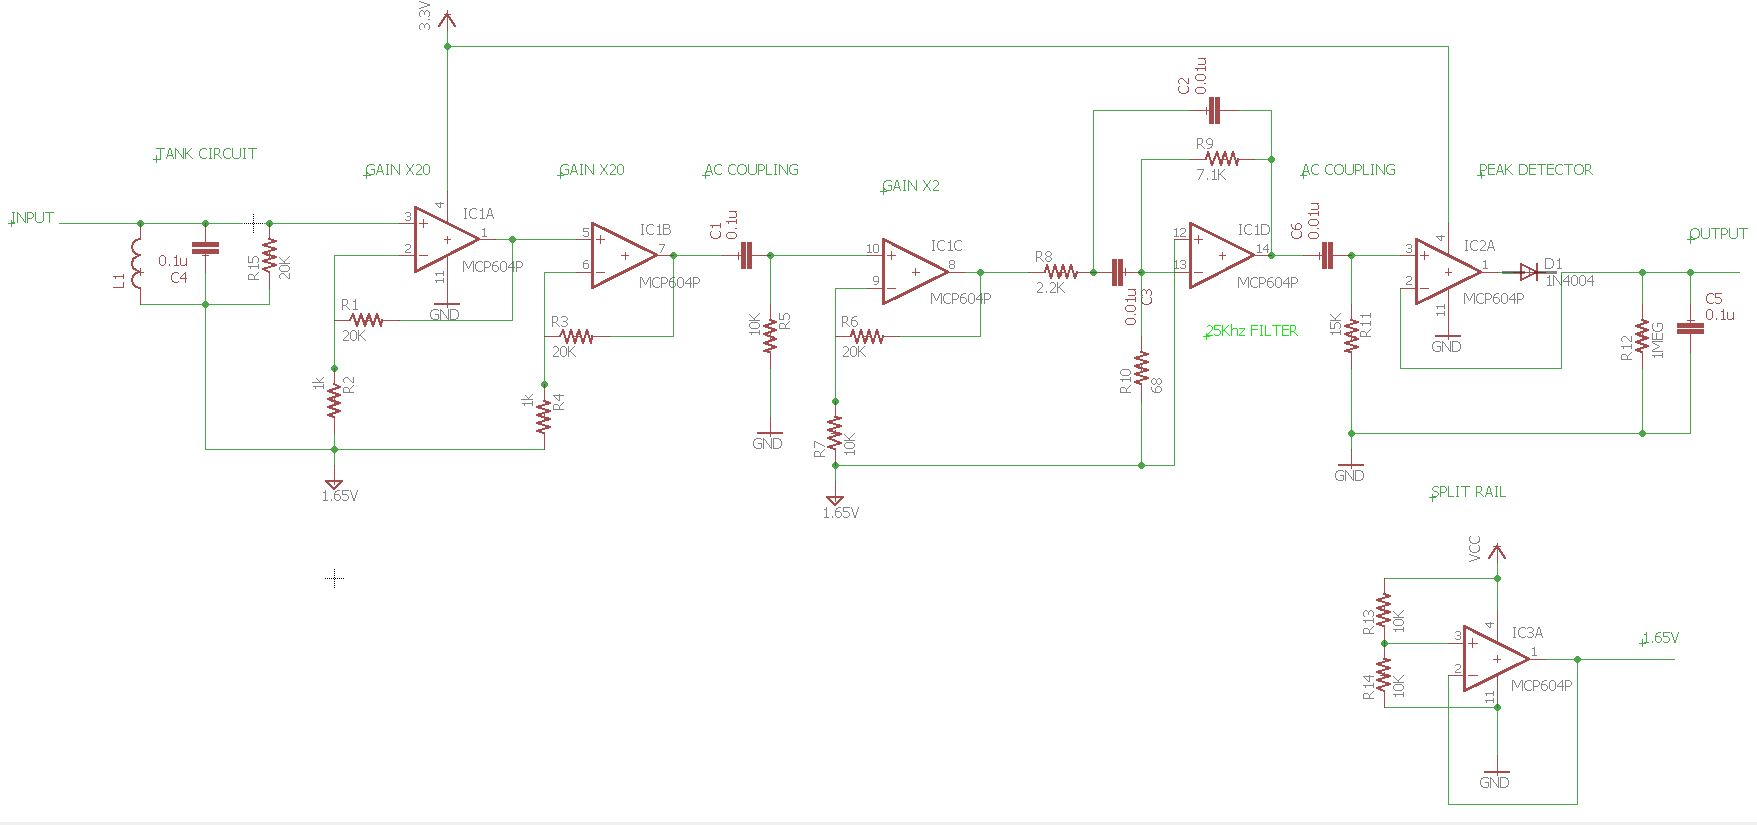
\includegraphics[scale=0.40]{TANK-CIRCUIT.JPG}
    \caption{Schematic of the circuit used to detect trackwires in AT-M6's.}
    \label{Trackwire circuit}
\end{figure}


Similarly, the beacon detector had to pick up a 2kHz signal, and attenuate all else with a band pass filter. This all had to be done with the caveat of picking up the signal from at least 6' away.

One interesting part of our beacon detector was to use a comparator to rail the input signal. This allowed us to remove two gain stages, greatly simplifying our circuit.

\begin{figure}[H]
    \centering
    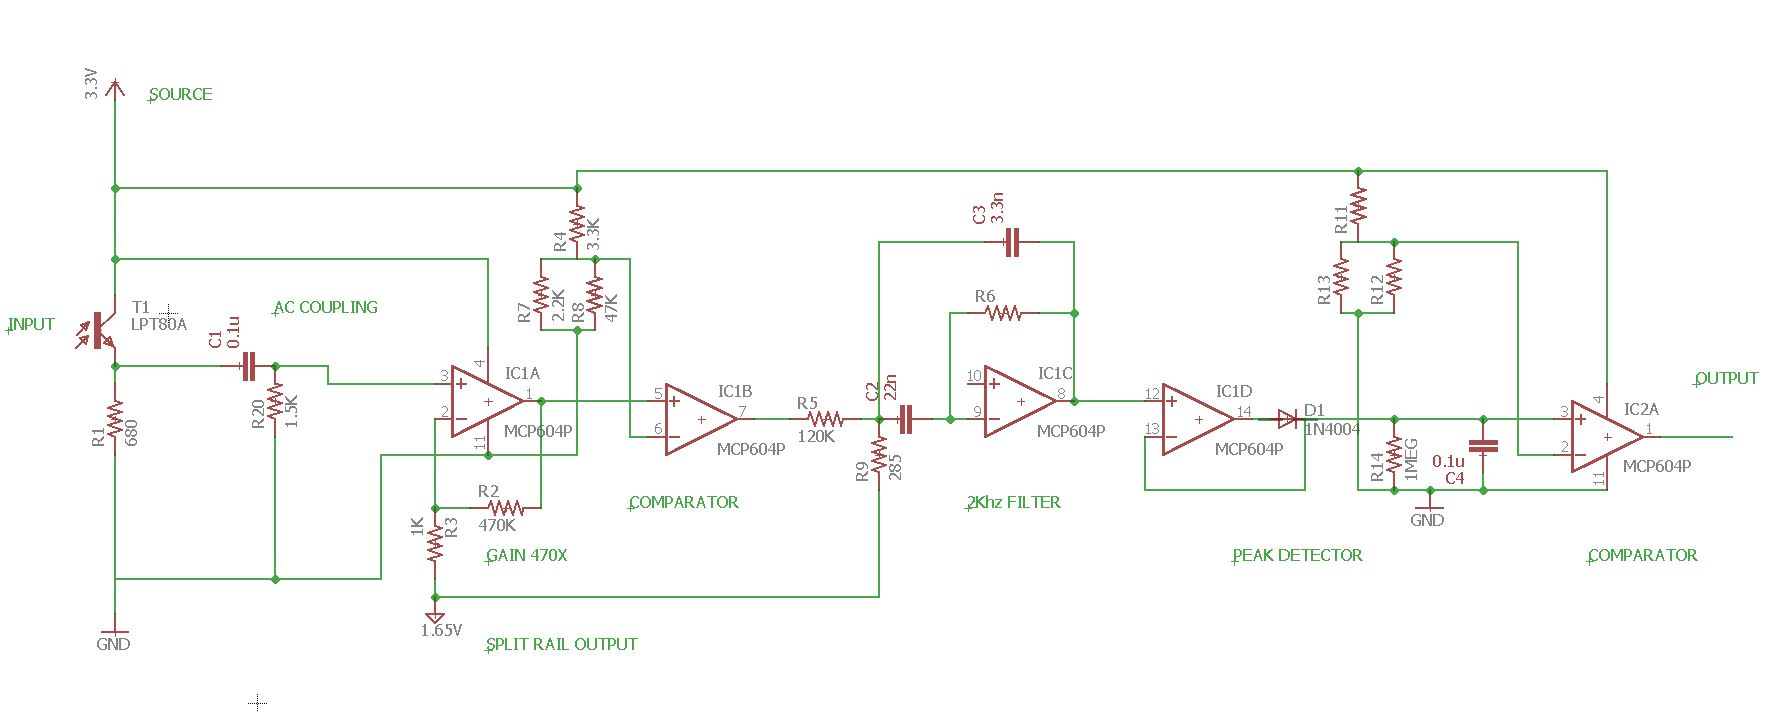
\includegraphics[scale=0.40]{BEACON_DETECTOR.JPG}
    \caption{Schematic of the circuit used to detect the Ren beacon.}
    \label{beacon detector}
\end{figure}

The other boards consisted of the sensor distribution boards, which all had some similarity with each other. These boards included the button distribution board, and the tape sensor distribution board, both shown in Figures \ref{button distro} and \ref{tape sensor distro}.

\begin{figure}[H]
    \Centering
    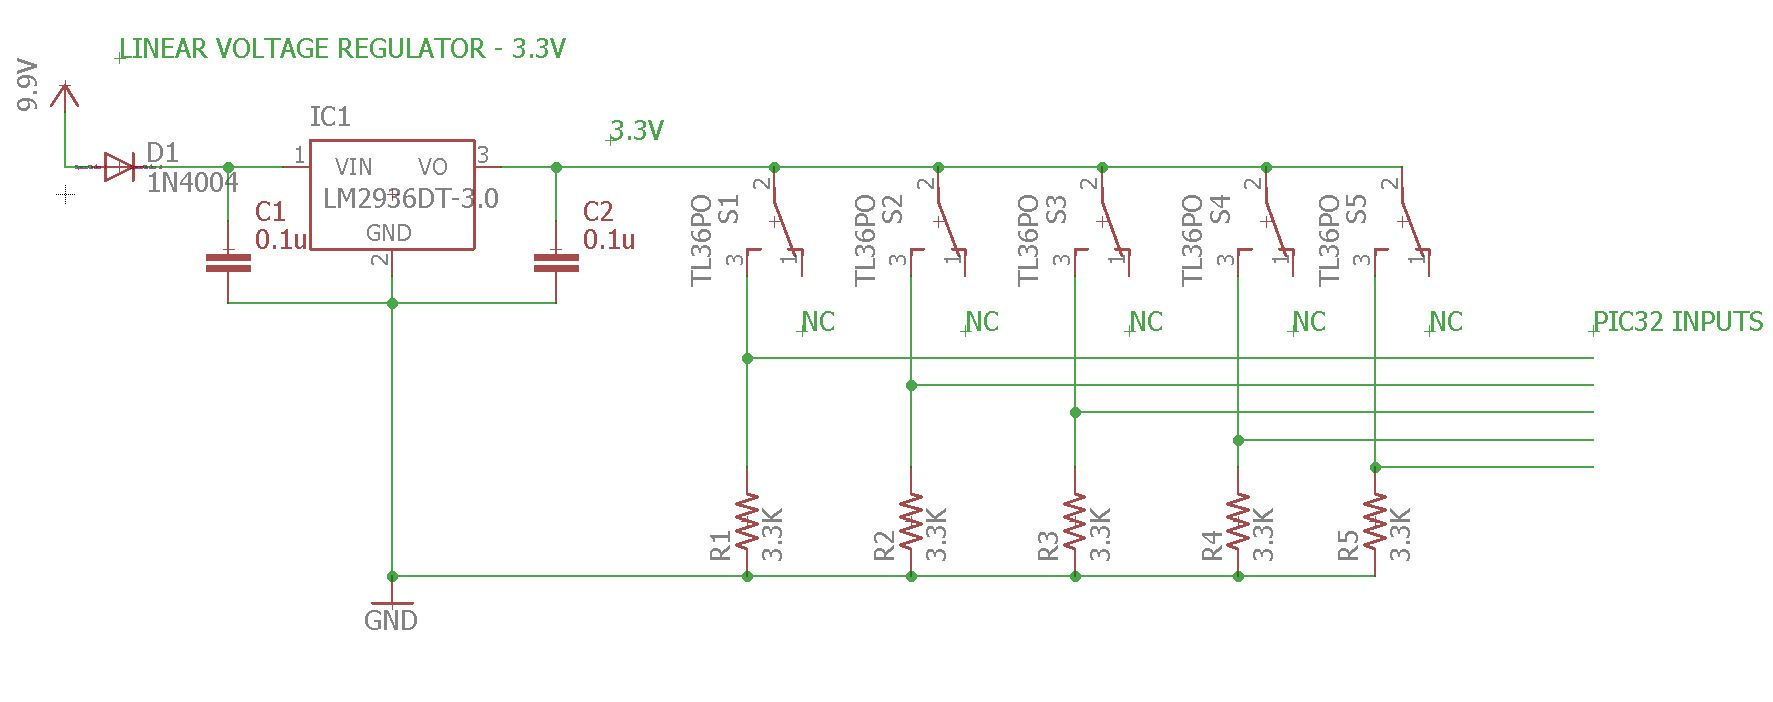
\includegraphics[scale = 0.5]{BUTTON-DISTRIBUTION-BOARD.JPG}
    \caption{ Switch distribution board. The source of the 9.9V in the schematic is the UNO power shield, as with all other boards}
    \label{button distro}
\end{figure}

\begin{figure}[H]
    \Centering
    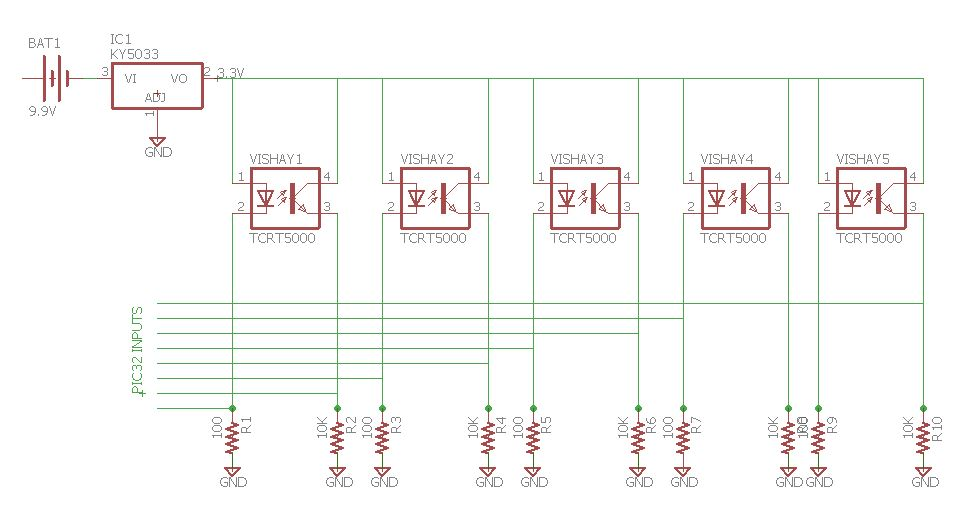
\includegraphics[scale = 0.5]{VishayDistro.JPG}
    \caption{The Vishay tape sensor distribution board.}
    \label{tape sensor distro}
\end{figure}

The IR sensors worked as follows: current was fed through an LED which output an infrared beam, on the other sides of the sensor was a phototransistor which would output a current. If the light from the LED reflects off the ground then the sensor is over a white patch of field, and the sensor outputs a DC value to the UNO, if the light doesn't reflect it means the sensor is over a patch of black tape. These elements are shown in the schematic above.

\subsection*{\textit{Setbacks}}

There were very few setbacks in the prototyping of electrical modules. The power/sensor distribution boards were prototyped fairly quickly, and soldering them onto perfboard was painless. The major setback we faced was with the trackwire detector. Our signal of interest lied at about 25kHz, however the motors produced very broadband noise. Our original plan was to add a second-order Butterworth Bandpass filter to our circuit created during the analog circuit lab.

The first iteration yielded the expected results so we proceeded to solder the circuit onto a perfboard. Upon completion of the soldering, we come to see that the circuit did not function as expected. The problem appeared to be that the trackwire detector was self oscillating. Our first instinct was to re-flow all solder joints and solder bridges to make sure they were in the right place. When, we were sure that the circuit we soldered was identical to what was on the breadboard, we compared results before and after re-flowing. The results remained unchanged. Out of curiosity we went back to examine the prototyped circuit on the breadboard. Needless to say, we found that circuit to be oscillating as well. The problem persisted even when there was no output from the filter stage going into the gain stage. Now, we knew it was not a soldering problem. To try to isolate the bug, we began testing each stage individually. We were able to detect that the filter stage was working as expected. When testing the gain stage directly after the filter, we saw the self oscillation again. Our first impulse was to scrap the gain stage and proceed without it. This did not eliminate the the oscillations. To remedy this, we added a buffer before the AC coupling but still produced no positive results. No matter what we tried, the oscillations were still present. For some odd reason, we pick the breadboard off the table while it's still hooked up to the oscilloscope and see that the oscillations vanish. To our surprise, this was no fluke. Every time we would set the breadboard down the oscillations returned. We were still stumped on what the problem could be until one group suggested we add a quality killing resistor to the tank part of our trackwire detector. This immediately yielded the results we were waiting for. We then proceeded to solder up the exact same circuit as before with the addition of some AC coupling after the second gain stage, as well as a Quality Killing Resistor to the Tank circuit. The trackwire circuit then worked as we expected. This was the only major issues, but that is not to say we did not have a handful of minor issue. 

While attempting check off, we had a variety of minor electrical problems; the first one being that our beacon detection was not as sensitive as we wanted it to be. The way we planned for the robot to orient itself after all three AT-M6's were eliminated would not have worked with the phototransistor included in our lab kit. We were ready to try to implement an entirely different circuit until another team member suggested we use a Photo-Darlington because of its increased sensitivity. To do this we had to de-solder the photo transistor from the perfboard. To keep it from turning possible solution to huge problem, we decided to solder on female headers and switch the phototransistor in for the photo-Darlington in case it proved to be useless. Right away we saw that the change added about two feet of range. We could be anywhere on the game field and detect the beacon.

Another less frightening problem we came across was a finicky trackwire detector. We had no intention of re-flowing the wire that connected the inductor to the rest of the perfboard until we were attempting check off and completely missed all three AT-M6's. We immediately went to re-flow the inductor, which drastically improved performance.

On a similar note, we were having what appeared to be an over current problem. To fix this, we simply switched the power from UNO power distribution board to H-bridge from one side of the UNO to another.


\subsection*{\textit{Results}}
Despite the various setbacks we suffered, our method of implementation allowed for a great amount of wire management and location versatility. In total there were three distribution boards, two sensor circuits, and two H-bridges. 

% -------------------------------------------------- %
% -------------------- Software -------------------- %
% -------------------------------------------------- %

\section{Software:}
\subsection*{\textit{Introduction}}
This is where we taught our robot how to think. In essence the software that runs the robot is just a large hierarchical state machine (HSM). All of this runs on top of the Events and Services Framework, which was provided for us. The ES Framework allows us to easily set up events, which are recognizable changes such as a sensor output changing or entering a new state in a state machine, as well as services to respond to those events with custom code. The entire HSM is in fact one service which responds to all of our sensor events. In addition to the state machine and sensor services, we have a set of helper functions described in the \textit{Motion} module for actuating motors and servos.

\subsection{Sensor Services}
One unique choice we made was to do all of our sensor event detection inside of services called by timers. This has the distinct advantage of debouncing events for you with no added code. The cost of doing this is that it requires one timer per service, but we were not close to running out of timers. 

The Sensor service modules are:
\begin{itemize}
    \item \textit{BumperService}
    \item \textit{TapeSensorService}
    \item \textit{TrackwireService}
    \item \textit{BeaconService}
\end{itemize}

Shown below are the lines which enable the services to be called periodically.
\begin{lstlisting}
#define TIMER0_RESP_FUNC PostTapeSensorService 
#define TIMER1_RESP_FUNC PostBumperService
#define TIMER2_RESP_FUNC PostTrackwireService
#define TIMER3_RESP_FUNC PostBeaconService
\end{lstlisting}

For the \textit{BumperService} and \textit{TapeSensorService} modules we decided to allow public access to the last recorded state of the sensor. This gave us flexibility in our state machines, and made initialization of certain processes much simpler. For example, when booting up the bot, we want to make sure that the lift is at the origin. We have a switch which is pressed when the lift is bottomed out, and checking the state of this bumper at start-up is much cleaner than forcing an event to occur.

\subsection{The \textit{Motion} Module}
The Motion.c/h files provide a clean interface of helper functions which drive motors or actuate servos. This was essential to creating a readable state machine. Included with this module is a test-harness for testing all of our controllable elements. This proved crucial later on during state machine design while debugging.

\subsection{State Machine}
Our main HSM is three levels deep, and the top level is broken into three main stages: Bootup, Hunt ATM6, and Hunt Ren. This in effect describes the entire game. Inside of these sub state machines (SSM) is a mixture of deeper SSMs as well as raw states for controlling motion of the bot.

\begin{figure}[H]
    \centering
    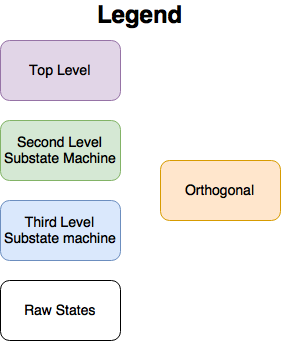
\includegraphics[scale=0.50]{hsm-legend.png}
    \caption{A legend for state machine diagrams.}
    \label{hsm legend}
\end{figure}


\subsubsection{Top Level}
\begin{figure}[H]
    \centering
    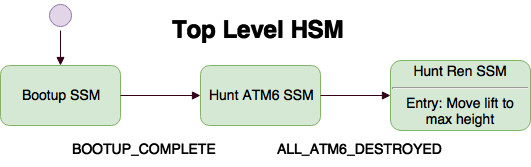
\includegraphics[scale=0.60]{hsm-top-level.png}
    \caption{Top level HSM diagram.}
    \label{hsm top level}
\end{figure}
Note that both of the state progression events in this level are created by the lower state machines, and are not created directly from sensor inputs. These events are \textbf{posted} back to this HSM, instead of simply changed inside the lower states.

Also important to note is the movement of the lift to max height at the entry of the Hunt Ren SSM. This is handled internally, and described in Section \ref{sec: hunt ren}.

\subsubsection{Bootup SSM}
\begin{figure}[H]
    \centering
    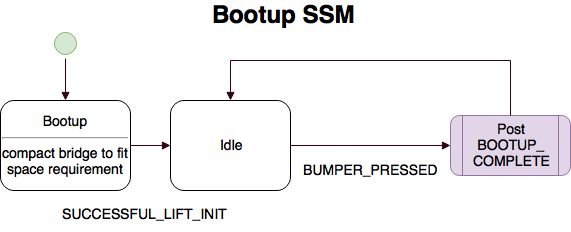
\includegraphics[scale=0.60]{bootup-ssm.png}
    \caption{Bootup SSM diagram.}
    \label{fig: bootup ssm}
\end{figure}
This SSM essentially puts the robot into a state which fulfills the space requirements of the project, and then waits for a bumper press before the robot actually starts its task.


\subsubsection{Hunt ATM6 SSM}
\begin{figure}[H]
    \centering
    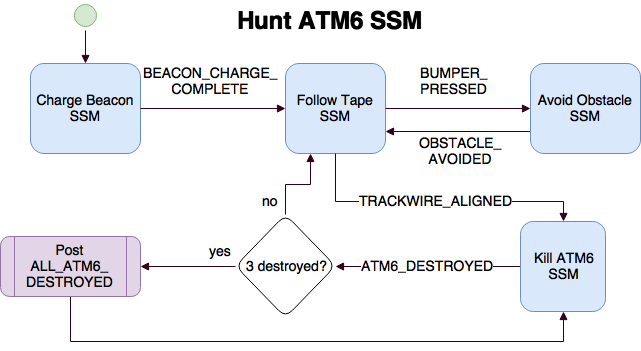
\includegraphics[scale=0.60]{hunt-atm6-ssm.png}
    \caption{Hunt ATM6 SSM Diagram.}
    \label{fig: hunt atm6 ssm}
\end{figure}
This SSM first tries to charge at Ren. This solves the problem of initial tape orientation. This is necessary in our case because we can only follow tape in one direction, and it is mathematically impossible to determine whether you are pointed inside or outside the play area if you are in the middle of the border tape.

After making a line for Ren, the bot eventually loses sight of the beacon and banks onto the side tape, or hits an object and turns out of its way onto the tape. This is handled inside the \textit{Charge Beacon SSM}. Either way. After running the charge beacon the bot starts following tape. While following tape, one of two things can happen, either a bumper event is received, meaning we need to dodge the obstacle, or a trackwire is detected meaning that we need to kill an ATM6.

Note that this SSM contains a counter which when incremented to three, posts an event to the top level signaling when to transition into the hunting Ren state.

\subsubsection{Charge Beacon SSM}
\begin{figure}[H]
    \centering
    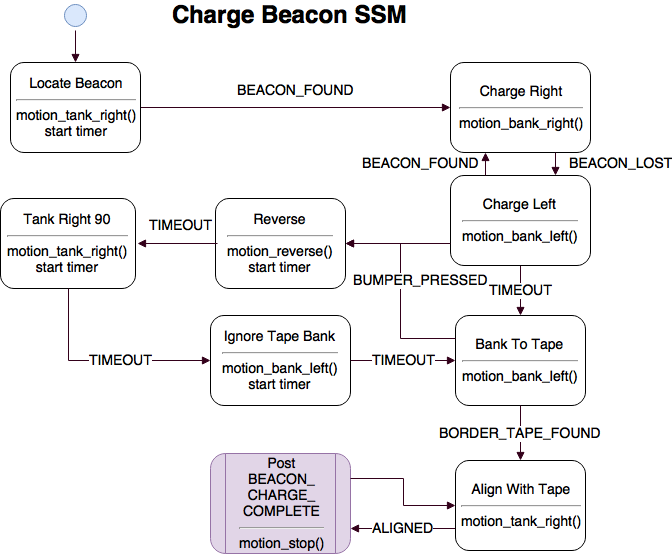
\includegraphics[scale=0.60]{charge-beacon-ssm.png}
    \caption{Charge Beacon SSM Diagram.}
    \label{fig: charge beacon ssm}
\end{figure}

This is the first SSM which contains only raw states and no SSMs, making it a bottom level SSM.

It first spins until a beacon is found. It then drives towards it, and oscillates between banking left and right waiting to lose and find it. This means that the bot follows the tightest possible line, but is offset to the left when charging towards the beacon. In the end this has little effect on performance as the offset is fairly minor. While tracking the beacon, if a bumper event is received, the bot will drive off to the left until tape is found. There is a period of time where tape is ignored, specifically for avoiding the tape in the middle of the field. After finding the border tape, this SSM aligns itself in such a way that the Follow Tape SSM can start following tape immediately. An event is posted signaling that the bot is aligned with tape, and that the charge is over.


\subsubsection{Follow Tape SSM}
\begin{figure}[H]
    \centering
    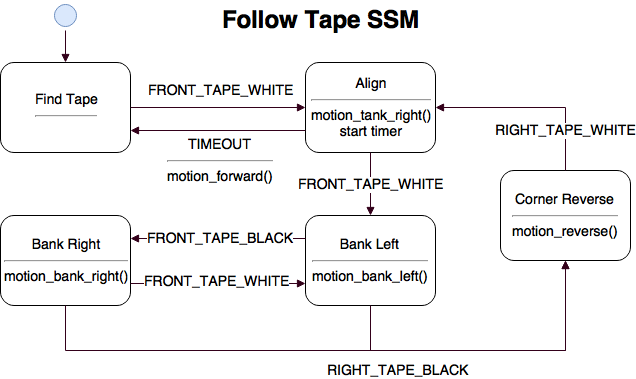
\includegraphics[scale=0.60]{follow-tape-ssm.png}
    \caption{Follow Tape SSM Diagram.}
    \label{fig: follow tape ssm}
\end{figure}

The following tape state machine following on the edge of a piece of tape by banking left and right. When the banks are set to reasonable speeds, this performs well and looks like a clean follow. When our right tape sensor is tripped, the bot is guaranteed to be in a corner. We back up slightly to account for overshoot, then tank until our front sensor is back at the edge of the tape. 

One advantage of this method is that you are essentially parallel with the tape at all times, which makes killing ATM6s much more consistent.

We also decided that Find Tape should leave the state of the drive wheels alone when entered. This provides the advantage of allowing the bot to find tape with any style of driving, but means that the caller of this state machine must specify a drive method (i.e. motion\_bank\_right()) before calling.

\subsubsection{Avoid Obstacle SSM}
\begin{figure}[H]
    \centering
    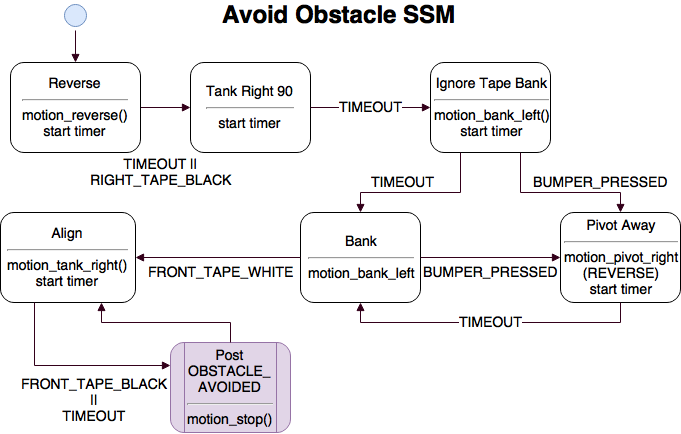
\includegraphics[scale=0.60]{avoid-obstacle-ssm.png}
    \caption{Avoid Obstacle SSM Diagram.}
    \label{fig: avoid obstacle ssm}
\end{figure}

This SSM is called whenever following tape, and a bumper event is received. This handles both dodging the Ren ship as well dodging the obstacle.

It simply backs up, turns right, and banks around the obstacle. For some time it ignores tape, before continuing with its bank while looking for tape. If at any point another bumper event is received the SSM pivots away from the obstacle, and continues banking.

\subsubsection{Kill ATM6 SSM}
\begin{figure}[H]
    \centering
    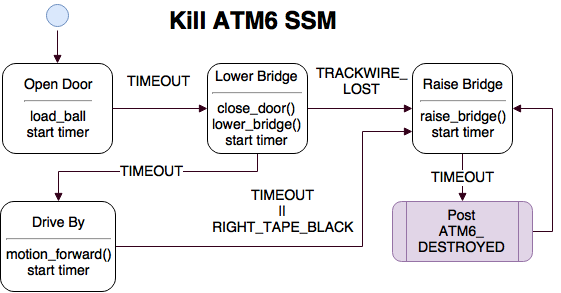
\includegraphics[scale=0.60]{kill-atm6-ssm.png}
    \caption{Kill ATM6 SSM Diagram.}
    \label{fig: kill ATM6 ssm}
\end{figure}

Our method for killing ATM6 is a very linear process:
\begin{enumerate}
    \item Open the detent servo (ball is loaded)
    \item Close the detent servo (stop extra balls)
    \item Lower the bridge (ball rolls through ATM6 hole)
    \item Raise the bridge
\end{enumerate}

Our method of tape following in conjunction with a relatively accurate trackwire detection method meant that this series of actions killed ATM6s very consistently, however we also included a Drive By state which simply drives forward after not killing the ATM6 after some amount of time. This worked for us because when we are misaligned with the trackwire the ball is already sitting against the ATM6, but is blocked from going into the hole.

\subsubsection{Hunt Ren SSM} \label{sec: hunt ren}
\begin{figure}[H]
    \centering
    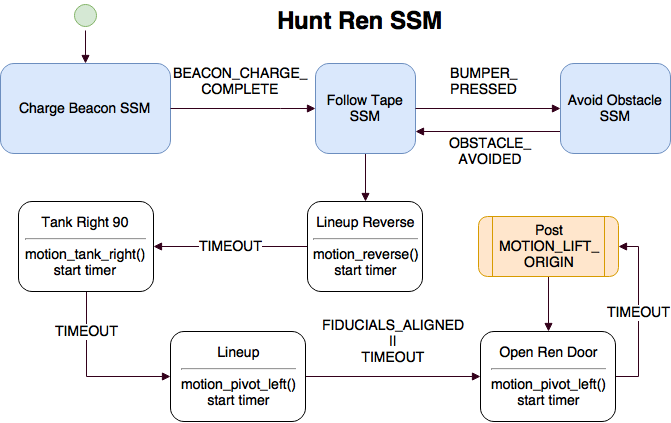
\includegraphics[scale=0.60]{hunt-ren-ssm.png}
    \caption{Hunt Ren SSM Diagram.}
    \label{fig: Hunt Ren ssm}
\end{figure}

Hunting Ren follows many of the first steps from Hunting ATM6s. We first charge the beacon until an obstacle is hit. By turning to the left after hitting an obstacle we have guaranteed a few key things. We either just moved around the obstacle, or we hit Ren, and then moved to tape. In both cases we have guaranteed that the next bump on our left bumper is at Ren! Doing this means we can use a simple timed pivot to line up with Ren consistently!

After pivoting to line up with Ren we can be in one of two cases, either the lift is still raising up to max height and the ball will fall into the Ren hole while moving up, or the lift is already maxed out. If the lift is maxed out already, we account for this by bringing the lift back to its minimum height, so the ball can roll in on its way down.

All of this was necessitated by significant problems with lift height consistency using timers alone. Using the max and minimum heights alone provided a guaranteed kill every time.

\subsubsection{Lift Control FSM}
\begin{figure}[H]
    \centering
    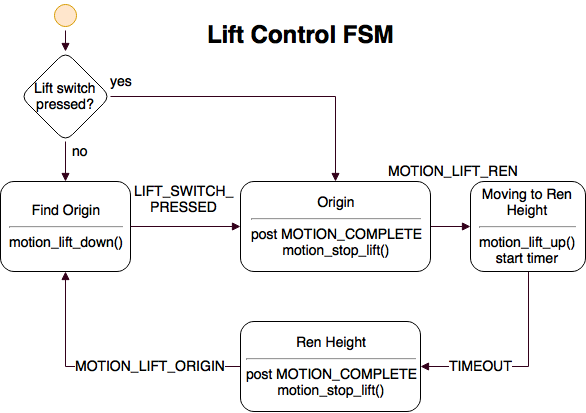
\includegraphics[scale=0.60]{lift-control-fsm.png}
    \caption{Lift Control FSM Diagram.}
    \label{fig: lift control fsm}
\end{figure}

We used an orthogonal state machine in our bot so that we could post to this FSM from any state within our main HSM. This was done implementing another service in our ES\_Configure.h, and changing our bumper service to post to two different services. We needed this FSM to see bumper events so that it could lower to a consistent height whenever a switch was pressed at its origin.
\begin{lstlisting}
#define NUM_DIST_LISTS 1
#if NUM_DIST_LISTS > 0 
#define DIST_LIST0 PostHSM, PostLiftControlFSM
#endif
\end{lstlisting}


\subsection*{\textit{Setbacks}}
Our main setbacks in software came mostly from silly bugs, and being married too closely to bad ideas. We ran into a significant slow down while trying to implement a box turn around obstacles. This proved to have many corner cases, and was generally unreliable with changing battery voltage levels, and wheel slippage.

Also before using the lift in only two positions, we attempted to play the game at a middle height. Because the lift had so much friction, and the amount of friction changed so rapidly, we could not count on this at all to deliver a reliable position. Ideally we would have had a method for mechanically detecting the height of the lift. Some ideas for this were switches inside the lift sleeve which would untrip as the bolt moved past them, as well as a switch connected by a string to the upper platform which would trip when the lift pulled the string taut.

\subsection*{\textit{Results}}

Our state machine delivered clean wins on a good percentage of fields. The failures of this machine are all caused by fairly rare placements of the obstacle. If an obstacle is placed awkwardly in the corner to the left of the Ren, we cannot line up with Ren. If we had more time, we would have implemented a way of lining up with Ren based on fiducial bump sensors to accommodate this scenario.

The other major shortfall is if there is a target in the corner, and an obstacle blocking it such that we would need to follow backwards in order to get to it.

\section*{Conclusion}

We are happy with our results in mech. Our bot was successful in completing the challenge. Furthermore we made a fairly unique design work, which is satisfying. The class of course has an outrageous amount of work but it gives you a real sense of satisfaction after making it through. Luke Skyscraper was a good friend to us, and cooperated with us to the best of his ability. Unfortunately for him, he was forcefully dismantled after being graded. The primary tools used for this were the heels of our shoes.

\appendix







%----- Templates ---------------------------------------------------------------

% \begin{eqnarray}
% 	\ul{h} &=& \sqrt{r_1^2+(x_1-r_2)^2} \\
% 	\ul{H} &=& \begin{bmatrix} \frac{x_1-r_2}{\sqrt{r_1^2 + (x_1 - r_2)^2}} & 0 & 0 \end{bmatrix}
% \end{eqnarray}

% \begin{figure}[H]
%     \centering
%     \includegraphics[scale=0.60]{ex2.png}
%     \caption{\E{x_2} over time.}
%     \label{ex2}
% \end{figure}


%----- Bibliography ------------------------------------------------------------

% \begin{thebibliography}{99}

% \bibitem{Name of Item}
% Proper citing text goes here
% \url{url_for_item}


% \end{thebibliography}

% \appendix
% \section{Name of Item}\label{label_for_item} 
% \url{ Link to Item} 


\end{document}